
\documentclass[../main.tex]{subfiles}

\begin{document}

\begin{figure}[p]
\centering
  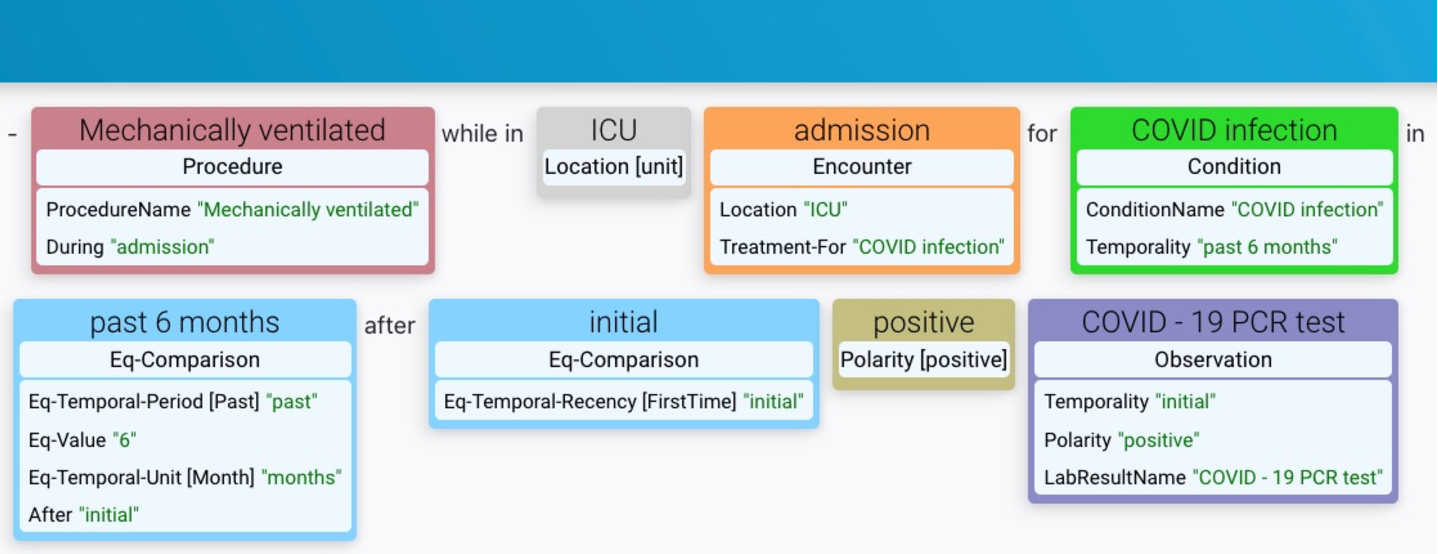
\includegraphics[scale=0.6]{figs/leafai2.pdf}  
\caption{Screenshot of a prototype web application for real-time entity and relation prediction on custom user input text.}
\label{fig_leafai}
\end{figure}

\begin{figure}[p]
\centering
  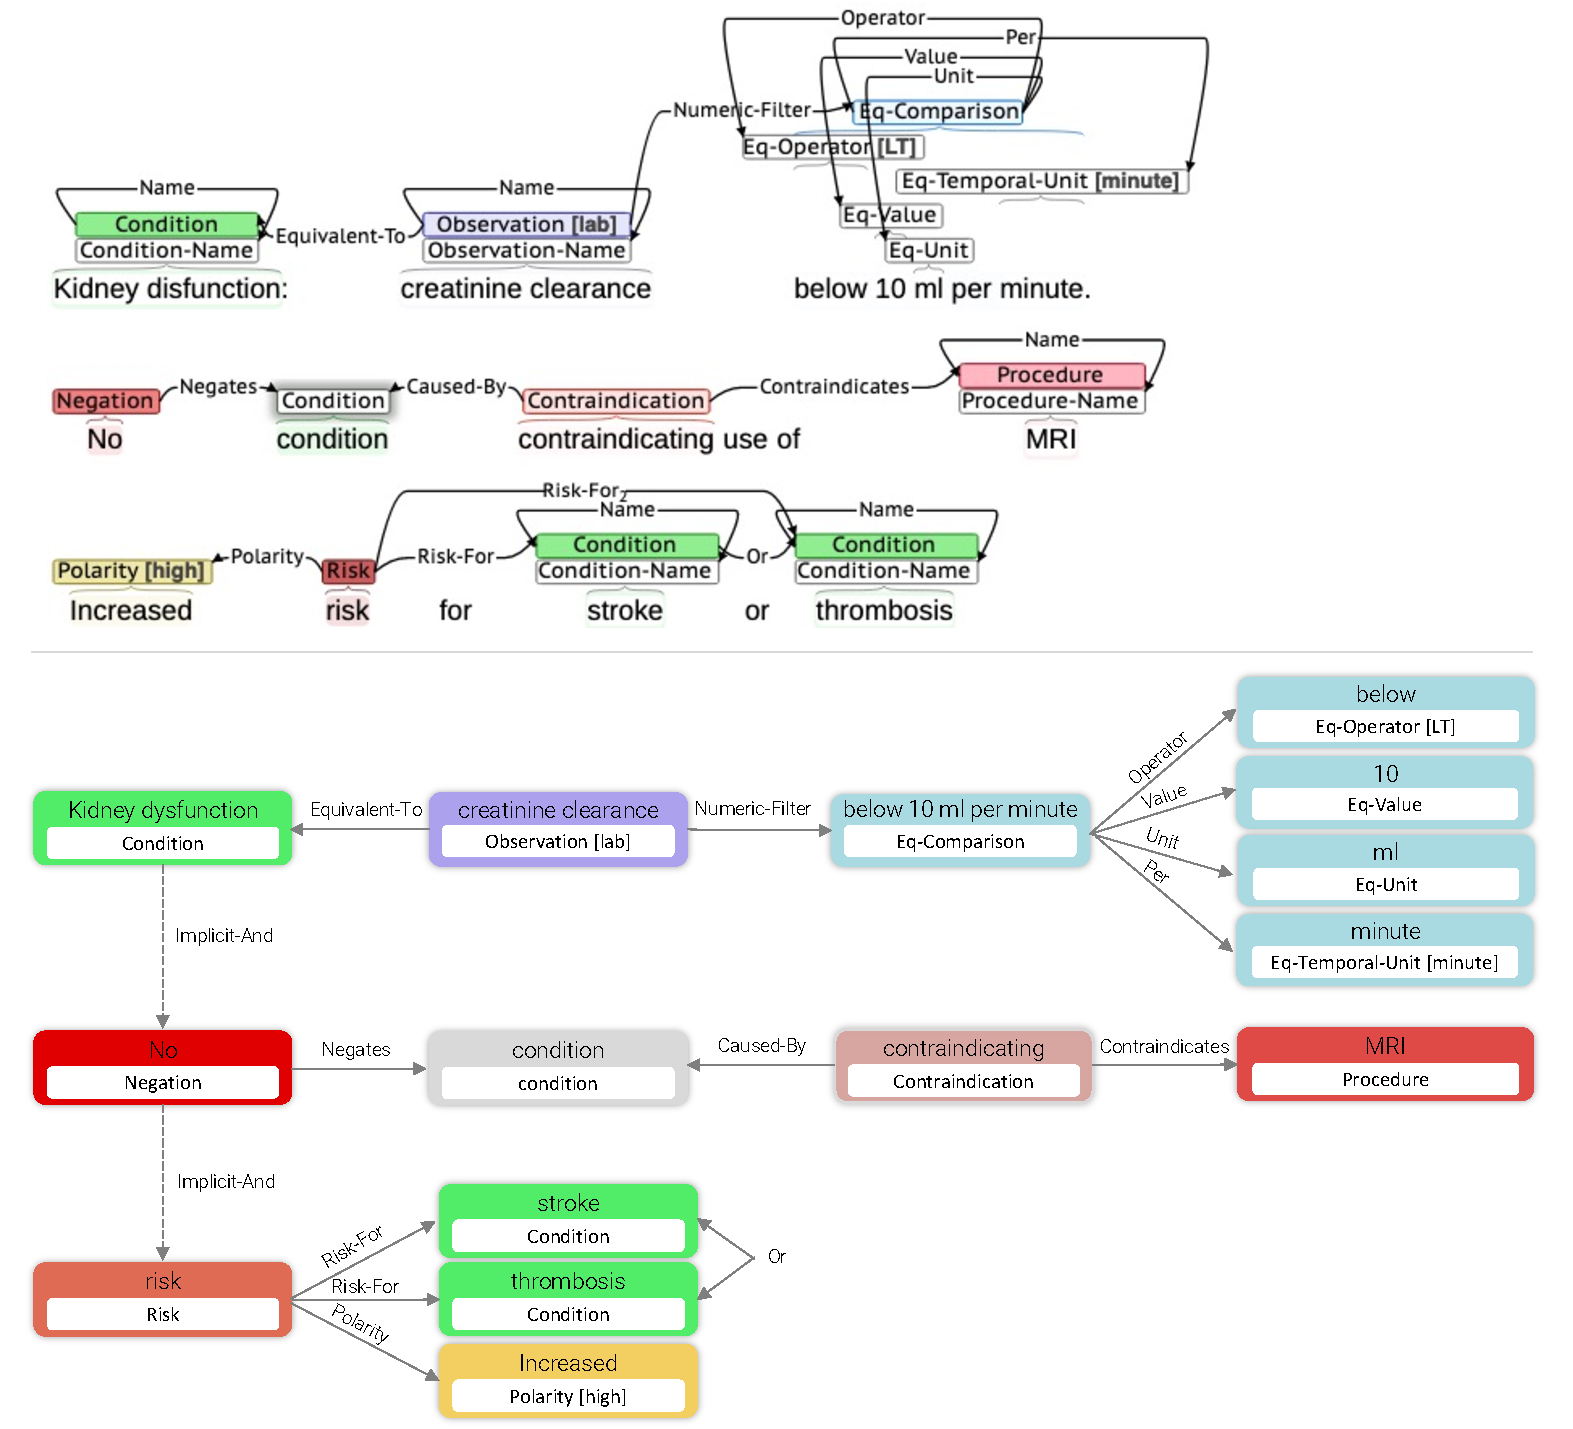
\includegraphics[scale=0.64]{figs/dag.pdf}  
\caption{Example of an LCT annotated document (top) transformed into a Directed Acyclical Graph (bottom). LCT entities and relations are readily transformable into tree, graph, or object-oriented representations used for query generation.}
\label{fig_dag}
\end{figure}

The LCT corpus is designed to facilitate query generation and question answering for real-world clinical trials and clinical research, specifically for a future version of the Leaf cohort discovery tool\cite{dobbins2019leaf}. Figure \ref{fig_dag} visualizes an example of a transformation of LCT annotated data into a Directed Acyclical Graph (DAG) structure, which can then be potentially compiled into SQL, FHIR, SPARQL, or other query methods. \\

\noindent To demonstrate the value and utility of the corpus, using the trained baseline Named Entity Recognition and Relation Extraction models, we developed a simple prototype web application to test named entity and relation prediction on unseen text. Figure \ref{fig_leafai} shows a screenshot of the models correctly predicting entities and relations on an input sentence not present in the LCT corpus. As can be seen, the models are able to predict entities and relations with very high accuracy on new text, demonstrating the power of the corpus. 

\subsection*{Limitations}
\noindent The LCT corpus is designed as a granular and robust resource of annotated eligibility criteria to enable models for entity and relation prediction as means of query generation. The corpus does have a number of limitations however which should be recognized. First, the corpus is largely singly annotated, with 119 of 1,006 documents (11\%) double annotated and reconciled, while double annotation is generally considered to be the gold standard in the NLP research community. As discussed in the Technical Validation section, the reasonably high F\textsubscript{1} score from experiments to evaluate NER when training on the singly annotated portion of the corpus suggests relative consistency of annotation across both single and double annotated documents. Additionally, entities in roughly half of the LCT corpus (493 documents) were automatically predicted, then manually corrected. This can potentially lead to data bias if predicted entities are not thoroughly reviewed and corrected by human annotators. Similar results from our experiments to detect differences in performance by training on the manually annotated portion versus the semi-automatically annotated portion (F\textsubscript{1} scores of 78.6\% and 80.0\%) suggest this may not be not a significant issue. Last, though the ultimate goal of the LCT corpus is to facilitate more accurate query generation, the corpus itself is not composed of queries by which it can be compared to similar corpora and thus cannot necessarily be proven to be more effective. Similarly, as we do not formally define a quantifiable means for measuring semantic representation within annotations, it is difficult to demonstrate that the LCT corpus enables more accurate query generation. \\

\subsection*{Future Work}
\noindent As discussed, evaluation of generated query accuracy and semantic representation in annotations is difficult and can potentially be done by different methods, such as ROUGE scoring \cite{lin2004rouge} to compare generated query syntax to expected syntax, or by including UMLS Concept identifiers \cite{bodenreider2004unified} within the LCT annotation schema and comparing the number of UMLS concepts to those found in other corpora. \\

\noindent Taking a different approach, in future work, we intend to evaluate the LCT corpus and query generation methods by evaluating generated queries in the context of real clinical trials which have taken place at the University of Washington (UW). As the UW EHR system maintains clinical trial enrollments and patient identifiers alongside clinical data, it is possible to query our EHR databases to compare patients who actually enrolled in clinical trials versus those found by our queries had they been run at the time of a given trial. We believe this means of evaluation is uniquely valuable as it uses real world clinical trials and EHR data while scoring queries by the accuracy of their ultimate results rather than less consequential factors such as syntax.

\end{document}